\chapter{Modélisation du système}
\section{Choix du modèle et conséquences}
	\subsection{Objectifs}
		L'objectif de ce chapitre est de développer une modélisation dynamique d'un robot humanoïde possédant une base mobile à roues omnidirectionnelles. 
		Ce modèle doit apporter un bon compromis entre fidélité vis à vis du comportement du robot réel et complexité, qui impacte de manière directe le temps de calcul.
		Notamment, il n'est pas nécessaire de modéliser tout les paramètres du robot : Représenter uniquement les dynamiques principales suffit à obtenir un contrôle précis du robot. 
		La section \ref{section.closedloop} détaillera les méthodes de compensation des éléments non modélisés.
	
		\fig{
			\label{fig.modele}
			\centering
			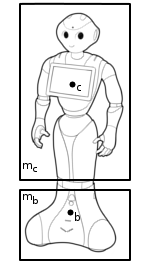
\includegraphics[width=2in]{modele.png}
			\caption{Représentation globale du modèle dynamique.}
		}
		
	\subsection{Avantages du modèle}
		
		Le choix se porte donc sur une modélisation dynamique d'un robot rigide multi-corps. 
		Le modèle présenté \rfi{fig.modele} comporte deux corps. Le premier est attaché à la base mobile, de masse $m_b$ et de position du centre de masse (CoM) $\bar{b}$.
		Le second modélise l'ensemble du reste du robot, de masse $m_c$ et de CoM $\bar{c}$.
		
		Le choix d'un modèle à deux corps permet de prendre en compte la rotation générale du corps du robot autour de la base mobile.
		Cette modélisation est pertinente dans le cas où les bras du robot ne génèrent que peu ou pas de moment d'inertie.
		Dans le cas contraire, nous considérerons que les effets parasites dû aux mouvements des bras pourront être compensés correctement par le schéma de contrôle en boucle fermée présenté en section \ref{section.closedloop}.
		Le choix de ce modèle est également conditionné par la répartition massique de la plate-forme expérimentale :
		Elle est principalement concentré en deux zones, qui correspondent aux corps choisis : la base mobile et le torse du robot.	
	
	\subsection{Inconvénients du modèle}
		
		Le choix d'un modèle rigide multi-corps implique que les éléments suivants ne seront donc pas modélisés :
		\liste{
			\item 	Les différentes élasticités. Les technologies d'actionnement utilisés sur la plate-forme expérimentale ne comportent pas d'élasticités notables.
				Le seul élément compliant est un ensemble de deux bandes élastiques attachés à l'articulation du roulis de la hanche permettant au robot de maintenir une posture droite en l'absence de contrôle du moteur.
				Cet élément est négligeable en terme de dynamique car la raideur associée est très faible.
			\item	Les jeux mécaniques présents sur le robot. Ceux-ci sont présents sur la plate-forme expérimentale, du fait de systèmes de réductions présents entre les moteurs et l'articulation basés sur un système d'engrenages.
				Les effets dynamiques parasites apportés par le jeu mécanique ne sont pas négligeables.
				Cependant, il peuvent être compensés de manière suffisamment efficace (plus de détails en section \ref{section.closedloop}) pour que cela soit transparent du point de vue de la commande présentée dans le chapitre \ref{chapitre.commande}.
			\item	Les glissements pouvant survenir entre les roues du robot et le sols ne sont pas modélisés. 
				Ceux-ci peuvent être néanmoins handicapant, car le système devient en partie non-observable en présence de glissement (plus de détails en section \ref{section.observateurbase}).
				Une solution a été apportée en section \ref{section.objectifs3roues} afin de limiter leurs possibilités d'apparition ainsi que leurs impacts sur la dynamique du robot.
			\item	Le nombre de corps choisi pour cette modélisation dynamique est nécessairement plus faible que le nombre de corps réels présents sur le robot, pour des raisons de complexité du modèle.
				Ainsi, tout les effets dynamiques ne pourront pas être représentés. Le choix du nombre de corps, et de leurs propriétés doit permettre de rendre négligeable les dynamiques non modélisées.
				Le développement d'une solution optimale du choix du nombre de corps et de leurs propriété est présenté en annexe \ref{annexe.choixmodele}.
		}
		

	\section{Modélisation dynamique}

		\subsection{Problème de complémentarité mixte}
		
			\subsubsection{Géométrie du robot}
			
				On considère le robot modélisé par deux masses-point $\bar{b}$ et $\bar{c}$ de masse associée $m_b$ et $m_c$. 
				Ces corps sont en contact avec le sol par l'intermédiaire de trois points $p_{frl}$ correspondant aux trois points de contact des roues avec le sol.
				La roue avant gauche correspond au point $p_r$, la roue avant droite au point $p_l$ et la roue arrière au point $p_f$.
				On considère que le système peut être dans quatre mode dynamique différents :
				\liste{
					\item Le robot ne bascule pas et les trois roues sont en contact avec le sol.
					\item Le robot est en rotation vers l'avant autour de l'axe défini par les deux roues avant. On note l'angle de rotation $\psi_f$. La roue arrière dans ce cas en l'air.
					\item Le robot est en rotation vers la gauche autour de l'axe défini par la roue avant gauche et la roue arrière. On note l'angle de rotation $\psi_l$. La roue avant droite dans ce cas en l'air.
					\item Le robot est en rotation vers la droite autour de l'axe défini par la roue avant droite et la roue arrière. On note l'angle de rotation $\psi_r$. La roue avant gauche dans ce cas en l'air.
				}
				Enfin, on ne considère aucune inertie associée à chaque corps. 
		
			\subsubsection{Cinématique directe}
			
				\subsubsubsection{Notations}
			
				Dans la suite, on considère un repère galiléen fixe orthonormé direct $\rep_w(O, \vec{x},\vec{y},\vec{z})$, $\vec{x}$ étant orienté vers l'avant du robot, $\vec{y}$ vers la gauche, et $\vec{z}$ vers le haut. 
				Ce repère est attaché au sol, $\vec{x}$ et $\vec{y}$ inclus dans le plan, et $\vec{z}$ orthogonal au sol. 
				
				Premièrement, on considère que la position des corps $\bar{c}$ et $\bar{b}$ correspond à la composition de trois éléments :
				Le premier définissant la position du robot par rapport à l'origine $c_0$ et $b_0$.
				Il est donc à noter que $c_0^{xy}=b_0^{xy}$.
				Le second est contrôlée par les moteurs du robot $\delta_c$. La base mobile ne possède pas de degrés de libertés par rapport à $b_0$.
				Le troisième dépendant de la rotation du système autour de ces différents axes.
				
				Afin de pouvoir écrire les équations cinématiques, nous avons besoin de définir différentes grandeurs dépendantes de la géométrie du robot. 
				
				$\forall i\in\{f,r,l\}$ :
				\liste{
					\item On note $\theta_i$ l'angle que fait le vecteur $\overrightarrow{b_0^{xy}~p_i^{xy}}$ avec l'axe $\vec{x}$. 
					      On note $\vec{n_i}$ l'axe résultant et l'axe orthogonal $\vec{t_i}=\vec{z} \times \vec{n_i}$.
					      $c_0$ et $b_0$ étant verticalement alignés, il en est de même pour le corps $\bar{c}$.
					      On note $\rep_i$ le repère $(O, \vec{n}_i, \vec{t}_i, \vec{z})$.
					\item On note $\phi_{i_b}$ et $\phi_{i_c}$ les angles que font respectivement les vecteurs $\overrightarrow{b_0^{t_iz}~p_i^{t_iz}}$ et $\overrightarrow{c_0^{t_iz}~p_i^{t_iz}}$ avec l'axe $\vec{z}$.
					\item $l_{b_i}$ et $l_{c_i}$ correspondent aux normes des vecteurs $\overrightarrow{b_0^{xyz}~p_i^{xyz}}$ et $\overrightarrow{c_0^{xyz}~p_i^{xyz}}$.
					\item $d_i$ correspond à la norme du vecteur $\overrightarrow{b_0^{xy}~p_i^{xy}}$, qui est la même concernant le corps $\bar{c}$.
					\item $h_b$ et $h_c$ correspondent à la composante selon l'axe $\vec{z}$ des vecteurs $\overrightarrow{b_0^{xyz}~p_i^{xyz}}$ et $\overrightarrow{c_0^{xyz}~p_i^{xyz}}$.
				}
				
				Enfin, on note $b$ et $c$ les positions commandées des corps par rapport à l'origine $O$ :
				\eqa{
					b^{xyz} &= b_0^{xyz}\\
					c^{xy} &= c_0^{xy}+\delta_c^{xy}  = b_0^{xy} + \delta_c^{xy} \\
					c^z &= c_0^z + \delta_c^z = b_0^z + h_c + \delta_c^z
				}
					
				\subsubsubsection{Equations cinématiques}
				
				Nous pouvons à présent écrire les équations cinématiques des corps $\bar{c}$ et $\bar{b}$ :
				\eqa{
				\label{eq.cin_cx}
					\bar{c}^x &= c^x + \somme{i\in\{f, r, l\}}{}{d_i\cos(\theta_i) + l_{c_i}\sin(\phi_{i_c}+\psi_i)\cos(\theta_i)}  \\
				\label{eq.cin_cy}
					\bar{c}^y &= c^y + \somme{i\in\{f, r, l\}}{}{d_i\sin(\theta_i) + l_{c_i}\sin(\phi_{i_c}+\psi_i)\sin(\theta_i)} \\
				\label{eq.cin_cz}
					\bar{c}^z &= c^z + \somme{i\in\{f, r, l\}}{}{-h_c + l_{c_i}\cos(\phi_{i_c}+\psi_i)} \\
				\label{eq.cin_bx}
					\bar{b}^x &= b^x + \somme{i\in\{f, r, l\}}{}{d_i\cos(\theta_i) + l_{b_i}\sin(\phi_{i_b}+\psi_i)\cos(\theta_i)}  \\
				\label{eq.cin_by}
					\bar{b}^y &= b^y + \somme{i\in\{f, r, l\}}{}{d_i\sin(\theta_i) + l_{b_i}\sin(\phi_{i_b}+\psi_i)\sin(\theta_i)} \\
				\label{eq.cin_bz}
					\bar{b}^z &= b^z + \somme{i\in\{f, r, l\}}{}{-h_b + l_{b_i}\cos(\phi_{i_b}+\psi_i)}
				}
				
				Nous aurons besoin également des équations cinématiques des points $p_{frl}$. $\forall i\in\{f,r,l\}$ :
				
				\eqa{
				\label{eq.cin_px}
					p_{i}^{x} &= b^{x} + d_{i}\cos(\theta_{i}) + l_{b_{i}}\sin(\phi_{i_b}+\psi_{i})\cos(\theta_{i}) \\
				\label{eq.cin_pz}
					p_{i}^{x} &= b^{y} + d_{i}\sin(\theta_{i}) + l_{b_{i}}\sin(\phi_{i_b}+\psi_{i})\sin(\theta_{i}) \\
				\label{eq.cin_py}
					p_{i}^{z} &= b^{z} - h_b + l_{b_{i}}\cos(\phi_{i_b}+\psi_{i})
				}
				
				\subsubsubsection{Hypothèse d'angles de basculements faibles}
				
				Dans la suite, afin de simplifier les formulations des équations de la dynamique, nous allons établir dès maintenant une hypothèse : Les angles $\psi_{frb}$ sont considérés proches de $0$.
				Dans le cas où le robot ne bascule pas, cela est une considtion exacte. Dans le cas où le robot bascule, on suppose le fait que l'angle de basculement reste faible ($<10$\degre).
				Nous pouvons donc réécrire les équations cinématiques \rf{eq.cin_cx}\rf{eq.cin_cy}\rf{eq.cin_cz}\rf{eq.cin_bx}\rf{eq.cin_by}\rf{eq.cin_bz} et \rf{eq.cin_px}\rf{eq.cin_py}\rf{eq.cin_pz} en utilisant une approximation du premier ordre :
				\eqa{
				\label{eq.cin_cx_appr}
					\bar{c}^x &= c^x + h_c\somme{i\in\{f, r, l\}}{}{\cos(\theta_i)\psi_i} \\
				\label{eq.cin_cy_appr}
					\bar{c}^y &= c^y + h_c\somme{i\in\{f, r, l\}}{}{\sin(\theta_i)\psi_i} \\
				\label{eq.cin_cz_appr}
					\bar{c}^z &= c^z + \somme{i\in\{f, r, l\}}{}{d_i\psi_i} \\
				\label{eq.cin_bx_appr}
					\bar{b}^x &= b^x + h_b\somme{i\in\{f, r, l\}}{}{\cos(\theta_i)\psi_i} \\
				\label{eq.cin_by_appr}
					\bar{b}^y &= b^y + h_b\somme{i\in\{f, r, l\}}{}{\sin(\theta_i)\psi_i} \\
				\label{eq.cin_bz_appr}
					\bar{b}^z &= b^z + \somme{i\in\{f, r, l\}}{}{d_i\psi_i}
				}

				\eqa{
					p_{frl}^{x} &= b^{x} - d_{frl}\cos(\theta_{frl}) \\
					p_{frl}^{y} &= b^{y} - d_{frl}\sin(\theta_{frl}) \\
					p_{frl}^{z} &= b^{z} - h_b + 2d_{frl}\psi_{frl} 
				}
			
			\subsubsection{Énergies cinétiques et potentielles}
			
			Afin d'exprimer les équations du mouvement du robot, nous allons utiliser la méthode Lagrangienne.
			Celle-ci est pertinente dans notre cas car elle est particulièrement adaptée à la formulation sans ambiguïtés de systèmes dynamiques soumis à des forces de contraintes, comme les forces de réactions dues au sol sur les roues. 
			Pour cela, il nous faut dans un premier temps écrire les équations des énergies cinétiques $T$ et potentielles $V$ du système :
			
			\eqa{
				T &= \frac{1}{2}m_b(\dot{\bar{b}}^{x^2} + \dot{\bar{b}}^{y^2} + \dot{\bar{b}}^{z^2}) + \frac{1}{2}m_c(\dot{\bar{c}}^{x^2} + \dot{\bar{c}}^{y^2} + \dot{\bar{c}}^{z^2}) \\
				V &= m_bg^x\bar{b}^x + m_cg^x\bar{c}^x + m_bg^y\bar{b}^y + m_cg^y\bar{c}^y + m_bg^z\bar{b}^z + m_cg^z\bar{c}^z \\
			}
			avec $g$ le vecteur gravité. Il est à noter que le repère $\rep_w$ étant attaché au sol, le vecteur gravité n'est pas forcément orienté selon la direction verticale $\vec{z}$, car le sol peut ne pas être horizontal.
			
			En dérivant les équations cinétiques \rf{eq.cin_cx_appr}\rf{eq.cin_cy_appr}\rf{eq.cin_cz_appr}\rf{eq.cin_bx_appr}\rf{eq.cin_by_appr}\rf{eq.cin_bz_appr}, nous pouvons exprimer les vitesses des corps $\bar{c}$ et $\bar{b}$ élevés au carré :
			\eqa{
				\dot{\bar{c}}^{x^2} &= \dot{c}^{x^2} + h_c^2\somme{i\in\{f, r, l\}}{}{\cos(\theta_i)^2\dot{\psi}_i^2} + 2h_c\dot{c}^x\somme{i\in\{f, r, l\}}{}{\cos(\theta_i)\dot{\psi}_i} \\
				\dot{\bar{c}}^{y^2} &= \dot{c}^{y^2} + h_c^2\somme{i\in\{f, r, l\}}{}{\sin(\theta_i)^2\dot{\psi}_i^2} + 2h_c\dot{c}^y\somme{i\in\{f, r, l\}}{}{\sin(\theta_i)\dot{\psi}_i}\\
				\dot{\bar{c}}^{z^2} &= \dot{c}^{z^2} + \somme{i\in\{f, r, l\}}{}{d_i^2\dot{\psi}_i^2} + 2\dot{c}^{z}\somme{i\in\{f, r, l\}}{}{d_i\dot{\psi}_i} \\
				\dot{\bar{b}}^{x^2} &= \dot{b}^{x^2} + h_b^2\somme{i\in\{f, r, l\}}{}{\cos(\theta_i)^2\dot{\psi}_i^2} + 2h_b\dot{b}^x\somme{i\in\{f, r, l\}}{}{\cos(\theta_i)\dot{\psi}_i} \\
				\dot{\bar{b}}^{y^2} &= \dot{b}^{y^2} + h_b^2\somme{i\in\{f, r, l\}}{}{\sin(\theta_i)^2\dot{\psi}_i^2} + 2h_b\dot{b}^y\somme{i\in\{f, r, l\}}{}{\sin(\theta_i)\dot{\psi}_i}\\
				\dot{\bar{b}}^{z^2} &= \dot{b}^{z^2} + \somme{i\in\{f, r, l\}}{}{d_i^2\dot{\psi}_i^2} + 2\dot{b}^{z}\somme{i\in\{f, r, l\}}{}{d_i\dot{\psi}_i}
			}
			
			
			
			
			
			
			
			
			
			///////////////////////////////////////
			
			Approximation ($\psi_{frb}$ proche de $0$) :
			\eqa{
				\bar{c}^x &= c^x + h_c\somme{i\in\{f, r, l\}}{}{\cos(\theta_i)\psi_i} \\
				\bar{c}^y &= c^y + h_c\somme{i\in\{f, r, l\}}{}{\sin(\theta_i)\psi_i} \\
				\bar{c}^z &= c^z + \somme{i\in\{f, r, l\}}{}{d_i\psi_i} \\
				\bar{b}^x &= b^x + h_b\somme{i\in\{f, r, l\}}{}{\cos(\theta_i)\psi_i} \\
				\bar{b}^y &= b^y + h_b\somme{i\in\{f, r, l\}}{}{\sin(\theta_i)\psi_i} \\
				\bar{b}^z &= b^z + \somme{i\in\{f, r, l\}}{}{d_i\psi_i}
			}
			
			Dérivation :
			
			\eqa{
				\dot{\bar{c}}^x &= \dot{c}^x + h_c\somme{i\in\{f, r, l\}}{}{\cos(\theta_i)\dot{\psi}_i} \\
				\dot{\bar{c}}^y &= \dot{c}^y + h_c\somme{i\in\{f, r, l\}}{}{\sin(\theta_i)\dot{\psi}_i} \\
				\dot{\bar{c}}^z &= \dot{c}^z + \somme{i\in\{f, r, l\}}{}{d_i\dot{\psi}_i} \\
				\dot{\bar{b}}^x &= \dot{b}^x + h_b\somme{i\in\{f, r, l\}}{}{\cos(\theta_i)\dot{\psi}_i} \\
				\dot{\bar{b}}^y &= \dot{b}^y + h_b\somme{i\in\{f, r, l\}}{}{\sin(\theta_i)\dot{\psi}_i} \\
				\dot{\bar{b}}^z &= \dot{b}^z + \somme{i\in\{f, r, l\}}{}{d_i\dot{\psi}_i}
			}
			
			Mise au carré (en prenant en considération que $\dot{\psi}_i\dot{\psi}_j=0$, $i\neq j$) :
			
			
			\eqa{
				\dot{\bar{c}}^{x^2} &= \dot{c}^{x^2} + h_c^2\somme{i\in\{f, r, l\}}{}{\cos(\theta_i)^2\dot{\psi}_i^2} + 2h_c\dot{c}^x\somme{i\in\{f, r, l\}}{}{\cos(\theta_i)\dot{\psi}_i} \\
				\dot{\bar{c}}^{y^2} &= \dot{c}^{y^2} + h_c^2\somme{i\in\{f, r, l\}}{}{\sin(\theta_i)^2\dot{\psi}_i^2} + 2h_c\dot{c}^y\somme{i\in\{f, r, l\}}{}{\sin(\theta_i)\dot{\psi}_i}\\
				\dot{\bar{c}}^{z^2} &= \dot{c}^{z^2} + \somme{i\in\{f, r, l\}}{}{d_i^2\dot{\psi}_i^2} + 2\dot{c}^{z}\somme{i\in\{f, r, l\}}{}{d_i\dot{\psi}_i} \\
				\dot{\bar{b}}^{x^2} &= \dot{b}^{x^2} + h_b^2\somme{i\in\{f, r, l\}}{}{\cos(\theta_i)^2\dot{\psi}_i^2} + 2h_b\dot{b}^x\somme{i\in\{f, r, l\}}{}{\cos(\theta_i)\dot{\psi}_i} \\
				\dot{\bar{b}}^{y^2} &= \dot{b}^{y^2} + h_b^2\somme{i\in\{f, r, l\}}{}{\sin(\theta_i)^2\dot{\psi}_i^2} + 2h_b\dot{b}^y\somme{i\in\{f, r, l\}}{}{\sin(\theta_i)\dot{\psi}_i}\\
				\dot{\bar{b}}^{z^2} &= \dot{b}^{z^2} + \somme{i\in\{f, r, l\}}{}{d_i^2\dot{\psi}_i^2} + 2\dot{b}^{z}\somme{i\in\{f, r, l\}}{}{d_i\dot{\psi}_i}
			}
			linéaire
			
			Énergie cinétique :
			
			\eqa{
				T &= \frac{1}{2}m_b(\dot{\bar{b}}^{x^2} + \dot{\bar{b}}^{y^2} + \dot{\bar{b}}^{z^2}) + \frac{1}{2}m_c(\dot{\bar{c}}^{x^2} + \dot{\bar{c}}^{y^2} + \dot{\bar{c}}^{z^2}) \\
				\nonumber T &= \frac{1}{2}m_b(\dot{b}^{x^2}+\dot{b}^{y^2}+\dot{b}^{z^2}) + \frac{1}{2}m_c(\dot{c}^{x^2}+\dot{c}^{y^2}+\dot{c}^{z^2}) + \frac{1}{2}(m_bh_b^2+m_ch_c^2)\somme{i\in\{f, r, l\}}{}{\dot{\psi}_i^2}\\
				\nonumber  &+ \frac{1}{2}(m_c+m_b)\somme{i\in\{f, r, l\}}{}{d_i^2\dot{\psi}_i^2}  + (m_ch_c\dot{c}^z+m_bh_b\dot{b}^z)\somme{i\in\{f, r, l\}}{}{d_i\dot{\psi}_i} \\
				&+ (m_bh_b\dot{b}^x+m_ch_c\dot{c}^x)\somme{i\in\{f, r, l\}}{}{\cos(\theta_i)\dot{\psi}_i} + (m_bh_b\dot{b}^y+m_ch_c\dot{c}^y)\somme{i\in\{f, r, l\}}{}{\sin(\theta_i)\dot{\psi}_i} \\
			}
			
			Énergie potentielle :
		
			\eqa{
				V &= m_bg^x\bar{b}^x + m_cg^x\bar{c}^x + m_bg^y\bar{b}^y + m_cg^y\bar{c}^y + m_bg^z\bar{b}^z + m_cg^z\bar{c}^z \\
				\nonumber V &= m_bg^xb^x + m_cg^xc^x + m_bg^yb^y + m_cg^yc^y + m_bg^zb^z + m_cg^zc^z \\
				\nonumber &+ (m_bg^x h_b + m_cg^x h_c)\somme{i\in\{f, r, l\}}{}{\cos(\theta_i)\psi_i} + (m_bg^y h_b + m_cg^y h_c)\somme{i\in\{f, r, l\}}{}{\sin(\theta_i)\psi_i} \\
				\nonumber &+(m_b+m_c)g^z\somme{i\in\{f, r, l\}}{}{d_i\psi_i}
			}
			
			Variables :
			\eq{
				q_i = \mat{b^x \\ b^y \\ b^z \\ c^x \\ c^y \\ c^z \\ \psi_f \\ \psi_r \\ \psi_l} 
			}
			
			On pose :
			\eqa{
				m_{hc} &= m_ch_c \\
				m_{hb} &= m_bh_b \\
				m_{q} &= m_{hc}h_c+m_{hb}h_b \\
				m_t &= m_c+m_b \\
				C_{\theta_i} &= \cos(\theta_i) \\
				S_{\theta_i} &= \sin(\theta_i)
			}
			
			Lagrange :
			
			\eqa{
				\frac{d}{dt}\frac{\partial L}{\partial \dot{q}_i} &=
				\mat{
					m_b\ddot{b}^x+m_bh_b\somme{i\in\{f, r, l\}}{}{\cos(\theta_i)\ddot{\psi}_i} \\
					m_b\ddot{b}^y+m_bh_b\somme{i\in\{f, r, l\}}{}{\sin(\theta_i)\ddot{\psi}_i} \\
					m_b\ddot{b}^z+m_bh_b\somme{i\in\{f, r, l\}}{}{d_i\ddot{\psi}_i} \\
					m_c\ddot{c}^x+m_ch_c\somme{i\in\{f, r, l\}}{}{\cos(\theta_i)\ddot{\psi}_i} \\
					m_c\ddot{c}^y+m_ch_c\somme{i\in\{f, r, l\}}{}{\sin(\theta_i)\ddot{\psi}_i} \\
					m_c\ddot{c}^z+m_ch_c\somme{i\in\{f, r, l\}}{}{d_i\ddot{\psi}_i} \\
					(m_q + m_td^2_f)\ddot{\psi}_f + m_{hb}(C_{\theta_f}\ddot{b}^x+S_{\theta_f}\ddot{b}^y-d_f\ddot{b}^z) + m_{hc}(C_{\theta_f}\ddot{c}^x+S_{\theta_f}\ddot{c}^y+d_f\ddot{c}^z) \\
					(m_q + m_td^2_r)\ddot{\psi}_r + m_{hb}(C_{\theta_r}\ddot{b}^x+S_{\theta_r}\ddot{b}^y-d_r\ddot{b}^z) + m_{hc}(C_{\theta_r}\ddot{c}^x+S_{\theta_r}\ddot{c}^y+d_r\ddot{c}^z) \\
					(m_q + m_td^2_l)\ddot{\psi}_l + m_{hb}(C_{\theta_l}\ddot{b}^x+S_{\theta_l}\ddot{b}^y-d_l\ddot{b}^z) + m_{hc}(C_{\theta_l}\ddot{c}^x+S_{\theta_l}\ddot{c}^y+d_l\ddot{c}^z)
				}
				,\\
				\frac{\partial L}{\partial q_i} &= \mat{
					m_bg^x \\
					m_bg^y \\
					m_bg^z \\
					m_cg^x \\
					m_cg^y \\
					m_cg^z \\
					(m_{hc} + m_{hb})\cos(\theta_f)g^x + (m_{hc} + m_{hb})\sin(\theta_f)g^y + m_td_fg^z \\
					(m_{hc} + m_{hb})\cos(\theta_r)g^x + (m_{hc} + m_{hb})\sin(\theta_r)g^y + m_td_rg^z \\
					(m_{hc} + m_{hb})\cos(\theta_l)g^x + (m_{hc} + m_{hb})\sin(\theta_l)g^y + m_td_lg^z
				}
			}
			
			Equations cinématiques :

			\eqa{
				p_{frl}^{x} &= b^{x} + d_{frl}\cos(\theta_{frl}) + l_{frl}\sin(\phi_{{frl}_b}+\psi_{frl})\cos(\theta_{frl}) \\
				p_{frl}^{x} &= b^{x} + d_{frl}\sin(\theta_{frl}) + l_{frl}\sin(\phi_{{frl}_b}+\psi_{frl})\sin(\theta_{frl}) \\
				p_{frl}^{z} &= b^{z} - h_b + l_{frl}\cos(\phi_{{frl}_b}+\psi_{frl})\\
			}
			
			Approximation ($\psi_{frb}$ proche de $0$) :

			\eqa{
				p_{frl}^{x} &= b^{x} - d_{frl}\cos(\theta_{frl}) \\
				p_{frl}^{y} &= b^{y} - d_{frl}\sin(\theta_{frl}) \\
				p_{frl}^{z} &= b^{z} - h_b + 2d_{frl}\psi_{frl} \\
			}
			Forces externes :
			
			\eqa{
				\frac{\partial p_{frl}^x}{\partial q_i} &= \mat{
					1\\
					0 \\
					0 \\
					0 \\
					0 \\
					0 \\
					0 \\
					0 \\
					0 \\
				},
				\frac{\partial p_{frl}^y}{\partial q_i} = \mat{
					0\\
					1 \\
					0 \\
					0 \\
					0 \\
					0 \\
					0 \\
					0 \\
					0 \\
				},
				\frac{\partial p_f^z}{\partial q_i} = \mat{
					0 \\
					0 \\
					1 \\
					0 \\
					0 \\
					0 \\
					2d_f \\
					0 \\
					0 \\
				},
				\frac{\partial p_r^z}{\partial q_i} = \mat{
					0 \\
					0 \\
					1 \\
					0 \\
					0 \\
					0 \\
					0 \\
					2d_r \\
					0 \\
				},
				\frac{\partial p_l^z}{\partial q_i} = \mat{
					0 \\
					0 \\
					1 \\
					0 \\
					0 \\
					0 \\
					0 \\
					0 \\
					2d_l \\
				},
			}
			
			Forces de contrainte : 
			
			\eq{
				\lambda = \mat{F_{p_{l}}^x \\ F_{p_{r}}^x \\ F_{p_{b}}^x \\ F_{p_{l}}^y \\ F_{p_{r}}^y \\ F_{p_{b}}^y \\ F_{p_{l}}^z \\ F_{p_{l}}^z \\ F_{p_{b}}^z}
			}
			
			Equation de Lagrange :
			
			\eqa{
				\nonumber \frac{d}{dt}\frac{\partial L}{\partial \dot{q}_i} - \frac{\partial L}{\partial q_i} &=
					  F_{p_{l}}^x\frac{\partial p_{l}^x}{\partial q_i}
					+ F_{p_{l}}^y\frac{\partial p_{l}^y}{\partial q_i}
					+ F_{p_{l}}^z\frac{\partial p_{l}^z}{\partial q_i} \\
					&+ F_{p_{r}}^x\frac{\partial p_{r}^x}{\partial q_i}
					+ F_{p_{r}}^y\frac{\partial p_{r}^y}{\partial q_i}
					+ F_{p_{r}}^z\frac{\partial p_{r}^z}{\partial q_i}\\
					&+ F_{p_{b}}^x\frac{\partial p_{b}^x}{\partial q_i}
					+ F_{p_{b}}^y\frac{\partial p_{b}^y}{\partial q_i}
					+ F_{p_{b}}^z\frac{\partial p_{b}^z}{\partial q_i}
			}
			
			Formulation généralisée :
			
			\eq{
				M \ddot{q} - f(q) = \tr{J}(q)\lambda
			}
			
			En identifiant :
			
			\eqa{
				M&=\mat{
					M_{bc} & M_{c\psi} \\ 
					\tr{M}_{c\psi} & M_\psi
				}, 
				M_{\psi} = \mat{
					m_q+m_td_f^2 & 0 & 0 \\
					0 & m_q+m_td_r^2 & 0 \\
					0 & 0 & m_q+m_td_l^2 
				}, \\
				M_{bc} &= \mat{
					m_b & 0 & 0 & 0 & 0 & 0 \\
					0 & m_b & 0 & 0 & 0 & 0 \\
					0 & 0 & m_b & 0 & 0 & 0 \\
					0 & 0 & 0 & m_c & 0 & 0 \\
					0 & 0 & 0 & 0 & m_c & 0 \\
					0 & 0 & 0 & 0 & 0 & m_c
				},
				M_{c\psi} = \mat{
					m_{hb}C_{\theta_f} & m_{hb}C_{\theta_r} & m_{hb}C_{\theta_l} \\
					m_{hb}S_{\theta_f} & m_{hb}S_{\theta_r} & m_{hb}S_{\theta_l} \\
					m_{hb}d_f & m_{hb}d_r & m_{hb}d_l \\
					m_{hc}C_{\theta_f} & m_{hc}C_{\theta_r} & m_{hc}C_{\theta_l} \\
					m_{hc}S_{\theta_f} & m_{hc}S_{\theta_r} & m_{hc}S_{\theta_l} \\
					m_{hc}d_f & m_{hc}d_r & m_{hc}d_l
				}, \\
				f(q) &= \mat{
					m_b g^x \\ 
					m_b g^y \\ 
					m_b g^z \\ 
					m_c g^x \\ 
					m_c g^y \\ 
					m_c g^z \\ 
					(m_{hc} + m_{hb})\cos(\theta_f)g^x + (m_{hc} + m_{hb})\sin(\theta_f)g^y + m_td_fg^z \\
					(m_{hc} + m_{hb})\cos(\theta_r)g^x + (m_{hc} + m_{hb})\sin(\theta_r)g^y + m_td_rg^z \\
					(m_{hc} + m_{hb})\cos(\theta_l)g^x + (m_{hc} + m_{hb})\sin(\theta_l)g^y + m_td_lg^z
				},\\
				\tr{J}(q) &= \mat{
					1 & 1 & 1 & 0 & 0 & 0 & 0 & 0 & 0 \\
					0 & 0 & 0 & 1 & 1 & 1 & 0 & 0 & 0 \\
					0 & 0 & 0 & 0 & 0 & 0 & 1 & 1 & 1 \\
					0 & 0 & 0 & 0 & 0 & 0 & 0 & 0 & 0 \\
					0 & 0 & 0 & 0 & 0 & 0 & 0 & 0 & 0 \\
					0 & 0 & 0 & 0 & 0 & 0 & 0 & 0 & 0 \\
					0 & 0 & 0 & 0 & 0 & 0 & 2d_f & 0 & 0 \\
					0 & 0 & 0 & 0 & 0 & 0 & 0 & 2d_r & 0 \\
					0 & 0 & 0 & 0 & 0 & 0 & 0 & 0 & 2d_l \\
				}
			}
			
			contraintes de complémentarité mixte :
			\eq{
				\forall (i, j) \in \{f,r,l\},~ i\neq j, 
				\lst{
					0 \le \psi_i \perp \psi_j \ge 0 \\
					0 \le \psi_i \perp F_i^z \ge 0 \\
					\psi_i F_i^x = 0 \\
					\psi_i F_i^y = 0
				}
			}
			
		\subsection{Les trois roues en contact avec le sol}

			On résout la complémentarité :
			\eq{
				\psi_{frl}=0
			}
			
			Le modèle dynamique devient :
\eq{
				M \ddot{q} - f(q) = \tr{J}(q)\lambda
			}
			
			En identifiant :
			
			\eqa{
				q_i &= \tr{\mat{b^x & b^y & b^z & c^x & c^y & c^z}} \\
				\lambda &= \tr{\mat{F_{p_{l}}^x & F_{p_{r}}^x & F_{p_{b}}^x & F_{p_{l}}^y & F_{p_{r}}^y & F_{p_{b}}^y & F_{p_{l}}^z & F_{p_{l}}^z & F_{p_{b}}^z}}\\
				F_{p_{l}}^z &\ge 0 \\
				M &= \mat{
					m_b & 0 & 0 & 0 & 0 & 0 \\
					0 & m_b & 0 & 0 & 0 & 0 \\
					0 & 0 & m_b & 0 & 0 & 0 \\
					0 & 0 & 0 & m_c & 0 & 0 \\
					0 & 0 & 0 & 0 & m_c & 0 \\
					0 & 0 & 0 & 0 & 0 & m_c
				},
				f(q) = \mat{
					m_b g^x \\ 
					m_b g^y \\ 
					m_b g^z \\ 
					m_c g^x \\ 
					m_c g^y \\ 
					m_c g^z 
				},\\
				\tr{J}(q) &= \mat{
					1 & 1 & 1 & 0 & 0 & 0 & 0 & 0 & 0 \\
					0 & 0 & 0 & 1 & 1 & 1 & 0 & 0 & 0 \\
					0 & 0 & 0 & 0 & 0 & 0 & 1 & 1 & 1 \\
					0 & 0 & 0 & 0 & 0 & 0 & 0 & 0 & 0 \\
					0 & 0 & 0 & 0 & 0 & 0 & 0 & 0 & 0 \\
					0 & 0 & 0 & 0 & 0 & 0 & 0 & 0 & 0 
				}
			}
			
			Principe du moment angulaire autour de l'axe $y$ et $x$ :
			\eqa{
				 m_b(\ddot{b}^z-g^z)b^x -m_b(\ddot{b}^x-g^x)b^z + m_c(\ddot{c}^z-g^z)c^x - m_c(\ddot{c}^x-g^x)c^z &= \somme{i\in\{f,r,l\}}{}{p_i^xF_i^z-p_i^zF_i^x} \\
				 m_b(\ddot{b}^z-g^z)b^y -m_b(\ddot{b}^y-g^y)b^z + m_c(\ddot{c}^z-g^z)c^y - m_c(\ddot{c}^y-g^y)c^z &= \somme{i\in\{f,r,l\}}{}{p_i^yF_i^z-p_i^zF_i^y}
			}
			
			Equation du mouvement sur l'axe $z$ :
			\eq{
				m_b(\ddot{b}^z-g^z) + m_c(\ddot{c}^z-g^z) = \somme{i\in\{f,r,l\}}{}{F_i^z}
			}
		
		
			Equation du CoP $d^{xy}$ :
			
			\eq{
				d^{xy} = \frac{\somme{i\in\{f,r,l\}}{}{p^{xy} \times F^{xy}}}{\somme{i\in\{f,r,l\}}{}{F_i^z}}
			}
			
			\eq{
				d^{xy} = \frac{m_b(\ddot{b}^z-g^z)b^{xy} -m_b(\ddot{b}^{xy}-g^{xy})b^z + m_c(\ddot{c}^z-g^z)c^{xy} - m_c(\ddot{c}^{xy}-g^{xy})c^z}  {m_b(\ddot{b}^z-g^z) + m_c(\ddot{c}^z-g^z)} \\
			}
			
			Les variables contrôlées sont directement $c^{xy}, b^{xy}$. $b^z$ est constant à la hauteur $h_b$ et on contraint $c^z$ à être constant à la hauteur $h_c$.
			De plus, la gravité est considérée selon l'axe z : $g=\tr{\mat{0, 0, -g}}$.
			
			\eq{
				d^{xy} = \frac{m_bgb^{xy} -m_b\ddot{b}^{xy}h_b + m_cgc^{xy} - m_c\ddot{c}^{xy}h_c}  {(m_b + m_c)g} 
			}
			
			Ce qui peut se réécrire, de façon conventionnelle :
			
			\eq{
				d^{xy} = \frac{m_bb^{xy}+m_cc^{xy}}{m_b+m_c} - \frac{m_bh_b\ddot{b}^{xy} + m_ch_c\ddot{c}^{xy}}{(m_b + m_c)g} \\
			}
			
			Les trois contrainte $F_{p_{frl}}^z \ge 0$ impliquent que $d^{xy}$ est dans le triangle défini par les trois points de contacts :
			\eqa{
				d^{xy} \times (p_r^{xy}-p_f^{xy}) &\ge 0 \\
				d^{xy} \times (p_l^{xy}-p_r^{xy}) &\ge 0 \\
				d^{xy} \times (p_f^{xy}-p_l^{xy}) &\ge 0
			}
		
		\subsection{Le robot bascule sur deux roues}

			On résout la complémentarité :
			\eq{
				\forall (i,j,k)\in\{f,r,l\}, i\neq j\neq k,~ \psi_{jk} = 0, F_i^{xyz} = 0
			}
			
			Le modèle dynamique devient :
			\eq{
				M \ddot{q} - f(q) = \tr{J}(q)\lambda
			}
			
			En identifiant :
			\eqa{
				q_i &= \tr{\mat{b^x & b^y & b^z & c^x & c^y & c^z & \psi_i}} \\
				\lambda &= \tr{\mat{F_{p_{j}}^x & F_{p_{k}}^x & F_{p_{j}}^y & F_{p_{k}}^y & F_{p_{j}}^z & F_{p_{k}}^z}}\\
				M &= \mat{
					m_b & 0 & 0 & 0 & 0 & 0 & m_{hb}C_{\theta_i} \\
					0 & m_b & 0 & 0 & 0 & 0 & m_{hb}S_{\theta_i} \\
					0 & 0 & m_b & 0 & 0 & 0 & m_{hb}d_i \\
					0 & 0 & 0 & m_c & 0 & 0 & m_{hc}C_{\theta_i} \\
					0 & 0 & 0 & 0 & m_c & 0 & m_{hc}S_{\theta_i} \\
					0 & 0 & 0 & 0 & 0 & m_c & m_{hc}d_i \\
					m_{hb}C_{\theta_i} & m_{hb}S_{\theta_i} & m_{hb}d_i & m_{hc}C_{\theta_i} & m_{hc}S_{\theta_i} & m_{hc}d_i & m_q+m_td_i^2
				},\\
				f(q) &= \mat{
					m_b g^x \\ 
					m_b g^y \\ 
					m_b g^z \\ 
					m_c g^x \\ 
					m_c g^y \\ 
					m_c g^z \\ 
					(m_{hc} + m_{hb})\cos(\theta_i)g^x + (m_{hc} + m_{hb})\sin(\theta_i)g^y + m_td_ig^z \\
				},\\
				\tr{J}(q) &= \mat{
					1 & 1 & 0 & 0 & 0 & 0 \\
					0 & 0 & 1 & 1 & 0 & 0 \\
					0 & 0 & 0 & 0 & 1 & 1 \\
					0 & 0 & 0 & 0 & 0 & 0 \\
					0 & 0 & 0 & 0 & 0 & 0 \\
					0 & 0 & 0 & 0 & 0 & 0 \\
					0 & 0 & 0 & 0 & 2d_j & 0 \\
					0 & 0 & 0 & 0 & 0 & 2d_k \\
				}
			}
			
			Principe du moment angulaire autour de l'axe $y$ et $x$ :
			\eqa{
				 \nonumber&m_b(\ddot{b}^z-g^z)b^x + m_bh_bd_i\ddot\psi_i\prt{b^x+h_b\cos(\theta_i)\psi_i} -m_b(\ddot{b}^x-g^x)b^z - m_bh_b\cos(\theta_i)\ddot\psi_ib^z\\
				 \nonumber+&m_c(\ddot{c}^z-g^z)c^x + m_ch_cd_i\ddot\psi_i\prt{c^x+h_c\cos(\theta_i)\psi_i} - m_c(\ddot{c}^x-g^x)c^z - m_ch_c\cos(\theta_i)\ddot\psi_ic^z\\
				 =& \somme{s\in\{j,k\}}{}{p_s^xF_s^z-p_s^zF_s^x}
			}
			\eqa{
				 \nonumber&m_b(\ddot{b}^z-g^z)b^y + m_bh_bd_i\ddot\psi_i\prt{b^y+h_b\sin(\theta_i)\psi_i} -m_b(\ddot{b}^y-g^y)b^z - m_bh_b\sin(\theta_i)\ddot\psi_ib^z\\
				 \nonumber+&m_c(\ddot{c}^z-g^z)c^y + m_ch_cd_i\ddot\psi_i\prt{c^y+h_b\sin(\theta_i)\psi_i} - m_c(\ddot{c}^y-g^y)c^z - m_ch_c\sin(\theta_i)\ddot\psi_ic^z\\
				 =& \somme{s\in\{j,k\}}{}{p_s^yF_s^z-p_s^zF_s^y}
			}
			
			Equation du mouvement sur l'axe $z$ :
			\eq{
				m_b(\ddot{b}^z-g^z) + m_bh_bd_i\ddot\psi_i + m_c(\ddot{c}^z-g^z) + m_ch_cd_i\ddot\psi_i = \somme{s\in\{j,k\}}{}{F_s^z}
			}
			
			Equation du CoP $d^{xy}$ :
			
			\eq{
				d^{xy} = \frac{\somme{i\in\{f,r,l\}}{}{p^{xy} \times F^{xy}}}{\somme{i\in\{f,r,l\}}{}{F_i^z}}
			}
			
			\eqa{
				\nonumber d^x &= \frac{m_b\prt{\ddot{b}^z-g^z+h_bd_i\ddot\psi_i}\prt{b^x+h_b\cos(\theta_i)\psi_i} - m_b\prt{\ddot{b}^x-g^x + h_b\cos(\theta_i)\ddot\psi_i}b^z}
				           {m_b(\ddot{b}^z-g^z) + m_c(\ddot{c}^z-g^z) + (m_bh_b+m_ch_c)d_i\ddot\psi_i} \\
				    &+ \frac{m_c\prt{\ddot{c}^z-g^z+h_cd_i\ddot\psi_i}\prt{c^x+h_c\cos(\theta_i)\psi_i} - m_c\prt{\ddot{c}^x-g^x + h_c\cos(\theta_i)\ddot\psi_i}c^z}
				           {m_b(\ddot{b}^z-g^z) + m_c(\ddot{c}^z-g^z) + (m_bh_b+m_ch_c)d_i\ddot\psi_i}
			}
			\eqa{
				\nonumber d^y &= \frac{m_b\prt{\ddot{b}^z-g^z+h_bd_i\ddot\psi_i}\prt{b^y+h_b\sin(\theta_i)\psi_i} - m_b\prt{\ddot{b}^y-g^y + h_b\sin(\theta_i)\ddot\psi_i}b^z}
				           {m_b(\ddot{b}^z-g^z) + m_c(\ddot{c}^z-g^z) + (m_bh_b+m_ch_c)d_i\ddot\psi_i} \\
				    &+ \frac{m_c\prt{\ddot{c}^z-g^z+h_cd_i\ddot\psi_i}\prt{c^y+h_b\sin(\theta_i)\psi_i} - m_c\prt{\ddot{c}^y-g^y + h_c\sin(\theta_i)\ddot\psi_i}c^z}
				           {m_b(\ddot{b}^z-g^z) + m_c(\ddot{c}^z-g^z) + (m_bh_b+m_ch_c)d_i\ddot\psi_i}
			}

			Les variables contrôlées sont directement $c^{xy}, b^{xy}$. $b^z$ est constant à la hauteur $h_b$ et on contraint $c^z$ à être constant à la hauteur $h_c$.
			De plus, la gravité est considérée selon l'axe z : $g=\tr{\mat{0, 0, -g}}$. Enfin, on considère $d_i=0$, ce qui correspond à négliger $d_i$ devant $h_b$ et $h_c$.
			
			\eqa{
				\nonumber d^x &= \frac{m_bg\prt{b^x+h_b\cos(\theta_i)\psi_i} + m_cg\prt{c^x+h_c\cos(\theta_i)\psi_i}}{(m_b+m_c)g} \\
				    &- \frac{m_bh_b\prt{\ddot{b}^x + h_b\cos(\theta_i)\ddot\psi_i}- m_ch_c\prt{\ddot{c}^x + h_c\cos(\theta_i)\ddot\psi_i}}{(m_b+m_c)g}
			}
			\eqa{
				\nonumber d^y &= \frac{m_bg\prt{b^y+h_b\sin(\theta_i)\psi_i} + m_cg\prt{c^y+h_c\sin(\theta_i)\psi_i}}{(m_b+m_c)g} \\
				    &- \frac{m_bh_b\prt{\ddot{b}^y + h_b\sin(\theta_i)\ddot\psi_i}- m_ch_c\prt{\ddot{c}^y + h_c\sin(\theta_i)\ddot\psi_i}}{(m_b+m_c)g}
			}
			
			Les deux contraintes $ F^z_{jk} \ge 0$ impliquent que $d^{xy}$ est dans le segment défini par les deux points de contact. 
			Pour assurer le maximum de robustesse, on choisi de contraindre le CoP au centre du segment :
			\eqa{
				d^x &= b^x + d_i\cos(\theta_i) \\
				d^y &= b^y + d_i\sin(\theta_i) 
			}
			
			On peut donc réécrire les équations précédente pour faire apparaitre la dynamique de $\psi_i$ par rapport à celles de $b$ et $c$ :
			\eqa{
				\label{eq.model_psi_x}
				\nonumber &(m_bh_b+m_ch_c)g\cos(\theta_i)\psi_i - (m_bh_b^2+m_ch_c^2)\cos(\theta_i)\ddot\psi_i \\
				=&~m_bh_b\ddot{b}^x + m_ch_c\ddot{c}^x - m_cg(c^x-b^x) - (m_c+m_b)gd_i\cos(\theta_i)
			}
			\eqa{
				\label{eq.model_psi_y}
				\nonumber &(m_bh_b+m_ch_c)g\sin(\theta_i)\psi_i - (m_bh_b^2+m_ch_c^2)\sin(\theta_i)\ddot\psi_i \\
				=&~m_bh_b\ddot{b}^y + m_ch_c\ddot{c}^y - m_cg(c^y-b^y) - (m_c+m_b)gd_i\sin(\theta_i)
			}
			
			Un rotation autour de l'axe $z$ de l'angle $\theta_i$ fait apparaitre, en combinant les équations \rf{eq.model_psi_x} et \rf{eq.model_psi_y} sous la forme \rf{eq.model_psi_n} $=cos(\theta_i)$\rf{eq.model_psi_x}$+\sin(\theta_i)$\rf{eq.model_psi_y} :
			\eq{
				\mat{c^x\\c^y} = \mat{\cos(\theta_i) & -\sin(\theta_i) \\ \sin(\theta_i) & \cos(\theta_i)} \mat{c^n \\c^t} 
			}
			\eq{
				\label{eq.model_psi_n}
				(m_bh_b+m_ch_c)g\psi_i - (m_bh_b^2+m_ch_c^2)\ddot\psi_i = m_bh_b\ddot{b}^n + m_ch_c\ddot{c}^n - m_cg(c^n-b^n) - (m_c+m_b)gd_i
			}
	\section{Modélisation de la dynamique future}
		\subsection{Nécessité de prédire le futur}

			- Les contraintes dynamiques sont trop fortes pour autoriser un contrôle sans prédiction du futur à haute accélération.

			- Démontrer en calculant les accélérations limites dans différents cas

			- Non nécéssité d'un modèle dynamique précis dans le futur (feedback, on ne calcule que la première commande)

			- Permet d'assurer une stabilité à long terme (quelques secondes)
		\subsection{Choix de la dynamique d'extrapolation}

			- Contraintes : Linéarité entre les variables / accélérations continues donc polynome d'ordre 3

			- Formulation de l'équation d'état

			- Calcul des dérivées

		\subsection{Formulation du modèle prédictif}

			- Formulation du modèle prédictif

			- Problème de controlabilité dans le cas de basculement.
			
			- Inversions de matrice